\section{Kiểm thử cho hệ thống}

Mục này trình bày chi tiết về quá trình kiểm thử được thực hiện trên hệ thống VieVu nhằm đảm bảo chất lượng, tính đúng đắn và độ ổn định của ứng dụng. Nội dung tập trung vào các phương pháp và kết quả kiểm thử ở các cấp độ khác nhau, bao gồm kiểm thử đơn vị và kiểm thử tích hợp API để xác minh logic nghiệp vụ phía máy chủ, đồng thời trình bày kết quả của các ca kiểm thử giao diện người dùng nhằm đánh giá sự tương tác thực tế và trải nghiệm người dùng trên ứng dụng di động.

\subsection{Kiểm thử các xử lý logic phía máy chủ}

Để đảm bảo các chức năng cốt lõi của hệ thống hoạt động chính xác, backend được kiểm thử với 2 phương pháp chính: kiểm thử đơn vị (unit testing) cho các hàm và module xử lý nghiệp vụ riêng lẻ, và kiểm thử tích hợp API (API integration testing) để xác minh sự tương tác giữa các thành phần và tính đúng đắn của các điểm cuối (endpoints) mà ứng dụng di động sẽ giao tiếp.

\subsubsection{Kiểm thử đơn vị}

\textbf{Phạm vi kiểm thử}

\noindent Phạm vi kiểm thử đơn vị của ứng dụng VieVu bao gồm kiểm thử các hàm xử lý và model của server Backend Python với FastAPI. 

\noindent
\textbf{Môi trường kiểm thử}

\noindent Môi trường kiểm thử đơn vị được thiết lập bằng cách sử dụng \texttt{pytest} \cite{pytest}, một framework kiểm thử phổ biến, mạnh mẽ và linh hoạt cho Python. \texttt{pytest} cung cấp nhiều tính năng nâng cao và cũng có khả năng khám phá và chạy các kiểm thử được viết bằng thư viện \texttt{unittest} \cite{unittest} tích hợp sẵn của Python. Trong dự án này, \texttt{pytest} được sử dụng để xác minh tính đúng đắn của các hàm xử lý logic cho những chức năng cốt lõi như gợi ý địa điểm, tổng hợp lịch trình từ tin nhắn và chức năng tìm kiếm tổng hợp của ứng dụng.

\noindent
\textbf{Kết quả kiểm thử}

\noindent Độ phủ và kết quả kiểm thử xử lý logic như Hình \ref{fig:pytest-testing}.

\begin{figure}[H]
    \centering  
    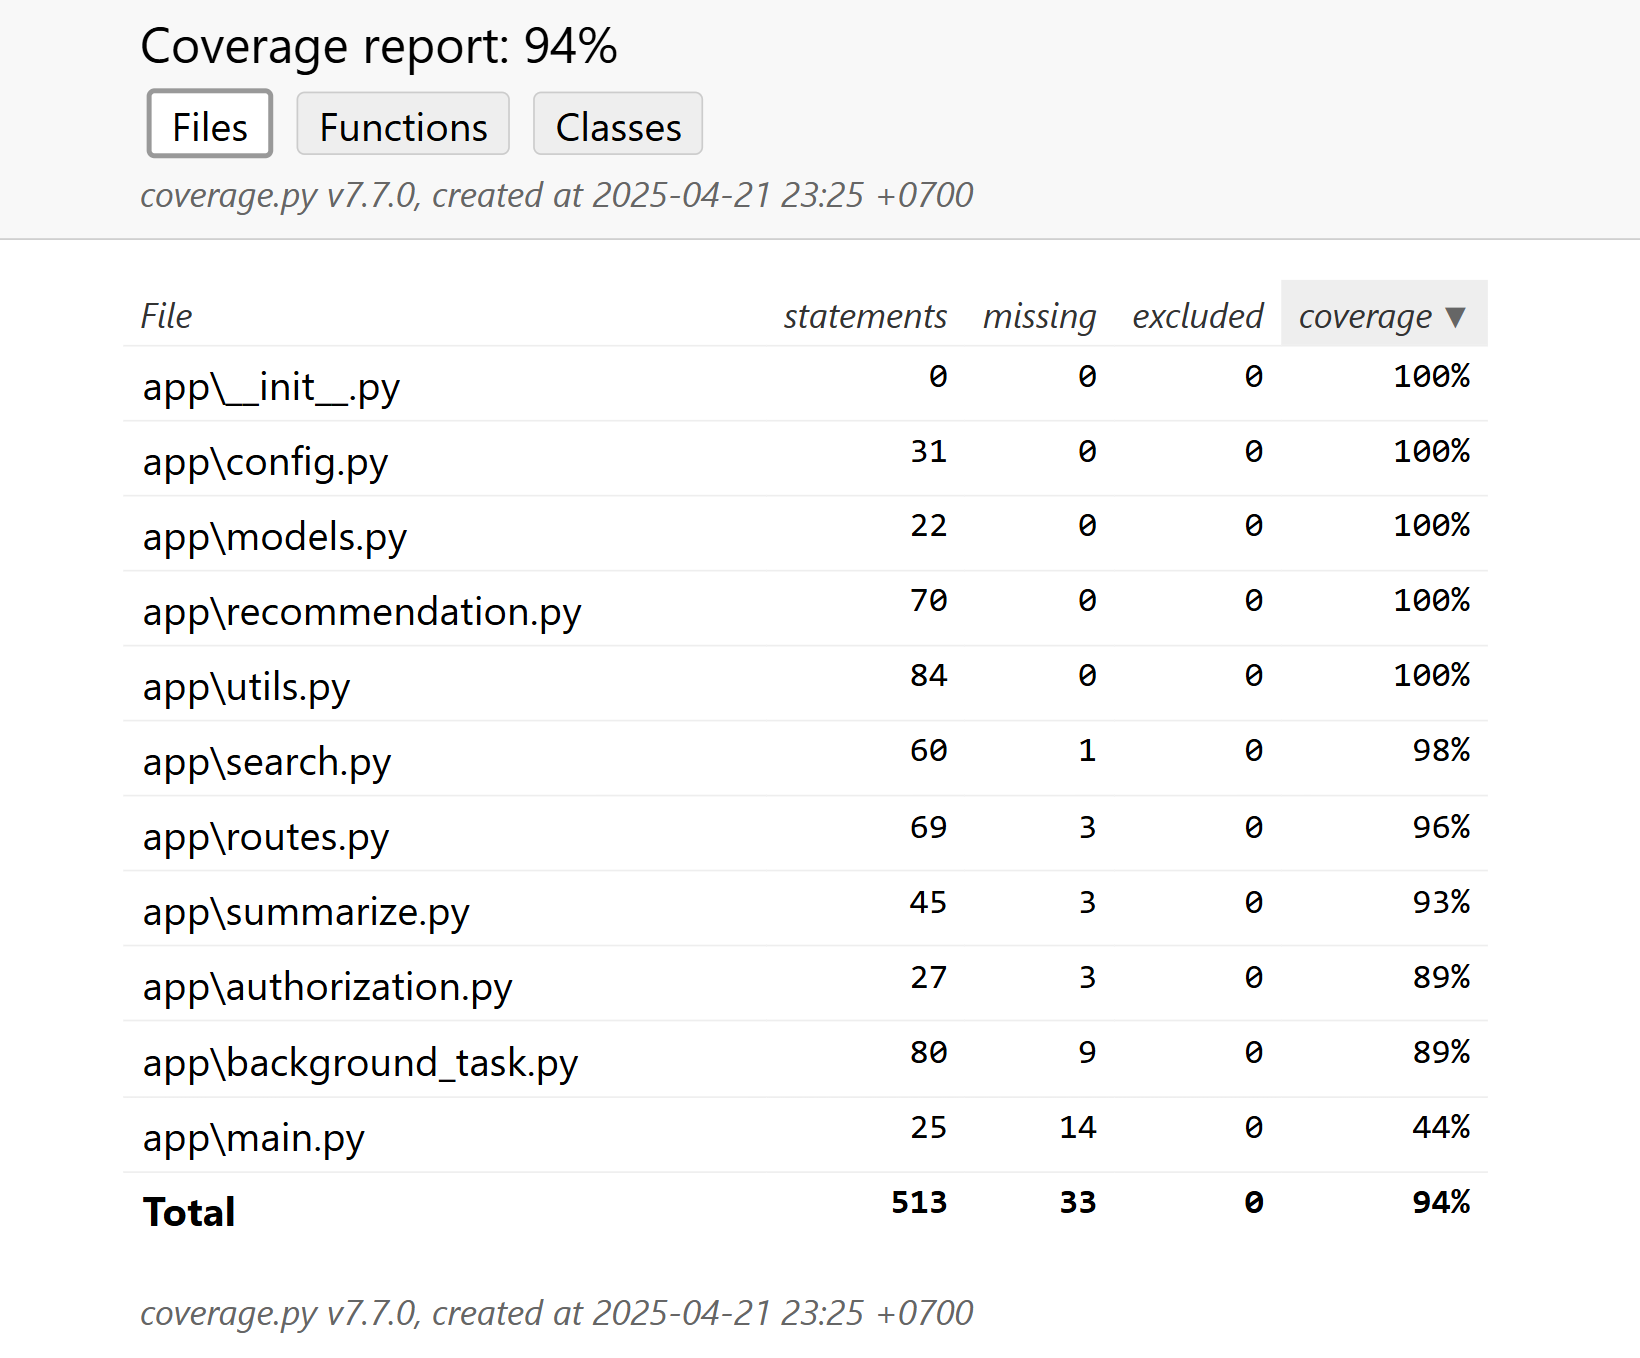
\includegraphics[width=1\textwidth]{figures/c4/unittest.png}
    \caption{Độ phủ kiểm thử xử lý logic với Pytest.}
    \label{fig:pytest-testing}
\end{figure}


\subsubsection{Kiểm thử API}

Chi tiết các ca kiểm thử (miêu tả, input và output) được mô tả dưới bảng sau \ref{tab:api-test-cases}. Hình \ref{fig:postman} dưới đây mô tả các API endpoint được kiểm thử với Postman\cite{postman}.  

\begin{figure}[H]
    \centering  
    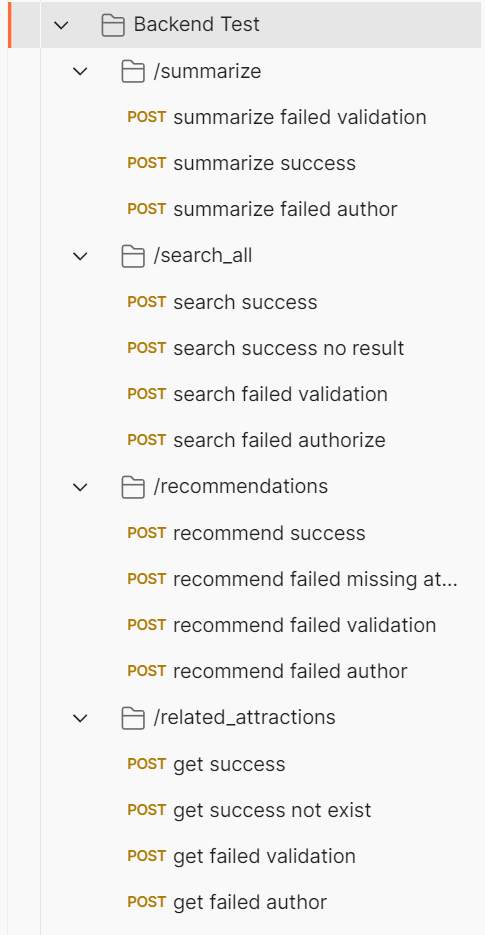
\includegraphics[width=0.5\textwidth]{figures/c4/api_test.png}
    \caption{Các API endpoint được kiểm thử với Postman.}
    \label{fig:postman}
\end{figure}


Bảng 4.2 mô tả một số kịch bảng kiểm thử API chính cho ứng dụng. 

\small
\begin{xltabular}{\textwidth}{|c|p{2cm}|X|X|c|}
    \caption{Các kịch bản kiểm thử API chính} \label{tab:api-test-cases} \\
    \hline
    \textbf{STT} & \textbf{API} & \textbf{Ca kiểm thử} & \textbf{Kết quả kỳ vọng} & \textbf{Tình trạng} \\
    \hline
    \endfirsthead
    
    % \multicolumn{5}{c}{\tablename\ \thetable{} (tiếp theo)} \\
    \hline
    \textbf{STT} & \textbf{API} & \textbf{Ca kiểm thử} & \textbf{Kết quả kỳ vọng} & \textbf{Tình trạng} \\
    \hline
    \endhead
    
    \hline
    %  \multicolumn{5}{r}{\textit{Tiếp trang sau}} \\
    \endfoot
    
    \hline
    \endlastfoot
     % --- API /search_all ---
     \multirow{4}{*}{1} & \multirow{4}{=}{\centering Tìm kiếm đa nền tảng} & Tìm kiếm thành công với từ khóa hợp lệ. & Hệ thống trả về mã 200 và danh sách kết quả đã được xếp hạng. & Đạt \\
     \cline{3-5}
      & & Tìm kiếm với từ khóa không có kết quả. & Hệ thống trả về mã 200 và danh sách kết quả rỗng. & Đạt \\
     \cline{3-5}
      & & Tìm kiếm với dữ liệu đầu vào không hợp lệ (sai kiểu dữ liệu `limit`). & Hệ thống trả về mã lỗi 422 và thông báo lỗi validation. & Đạt \\
     \cline{3-5}
      & & Tìm kiếm khi chưa xác thực (thiếu header `Authorization`). & Hệ thống trả về mã lỗi 401 và thông báo cần xác thực. & Đạt \\
     \hline
 
     \multirow{4}{*}{1} & \multirow{4}{=}{\centering Đề xuất địa điểm} & Lấy đề xuất thành công với sở thích và danh sách ID hợp lệ. & Hệ thống trả về mã 200 và danh sách đề xuất được xếp hạng. & Đạt \\
     \cline{3-5}
      & & Lấy đề xuất với params `user\_preferences` thiếu thuộc tính. & Hệ thống trả về mã lỗi 500 và thông báo lỗi thiếu thuộc tính. & Đạt \\
     \cline{3-5}
      & & Lấy đề xuất với dữ liệu đầu vào không hợp lệ, thiếu `preferences`. & Hệ thống trả về mã lỗi 422 và thông báo lỗi validation. & Đạt \\
      \cline{3-5}
      & & Lấy đề xuất khi chưa xác thực (thiếu header `Authorization`). & Hệ thống trả về mã lỗi 401 và thông báo cần xác thực. & Đạt \\
     \hline
 
     \multirow{4}{*}{1} & \multirow{4}{=}{\centering Tìm địa điểm liên quan } & Lấy địa điểm liên quan thành công với ID hợp lệ. & Hệ thống trả về mã 200 và danh sách địa điểm liên quan. & Đạt \\
     \cline{3-5}
      & & Lấy địa điểm liên quan với `att\_id` không hợp lệ (sai kiểu dữ liệu). & Hệ thống trả về mã lỗi 422 và thông báo lỗi validation. & Đạt \\
     \cline{3-5}
      & & Lấy địa điểm liên quan với `att\_id` không tồn tại. & Hệ thống trả về mã 200 và danh sách địa điểm liên quan rỗng. & Đạt \\
      \cline{3-5}
      & & Lấy địa điểm khi chưa xác thực (thiếu header `Authorization`). & Hệ thống trả về mã lỗi 401 và thông báo cần xác thực. & Đạt \\
     \hline
 

     \multirow{3}{*}{5} & \multirow{3}{=}{\centering Tóm tắt hội thoại} & Tóm tắt thành công với dữ liệu hội thoại hợp lệ. & Hệ thống trả về mã 200, cấu trúc lịch trình (`data`) và văn bản tóm tắt (`reading`). & Đạt \\
     \cline{3-5}
      & & Tóm tắt với dữ liệu đầu vào không hợp lệ (sai định dạng ngày). & Hệ thống trả về mã lỗi 422 và thông báo lỗi validation. & Đạt \\
     \cline{3-5}
      & & Tóm tắt khi chưa xác thực (thiếu header `Authorization`). & Hệ thống trả về mã lỗi 401 và thông báo cần xác thực. & Đạt \\
     \hline
 
\end{xltabular}


\subsection{Kiểm thử tương tác người dùng trên giao diện ứng dụng}

Hệ thống VieVu thực hiện kiểm thử tương tác người dùng trên giao diện với các ca kiểm thử tính năng chính của hệ thống được báo cáo lại trong bảng \ref{tab:ui-test-cases}.

\small
\begin{xltabular}{\textwidth}{|c|p{5cm}|X|c|}
    \caption{Các kịch bản kiểm thử tương tác người dùng} \label{tab:ui-test-cases} \\
    \hline
    \textbf{STT} & \textbf{Ca kiểm thử} & \textbf{Kết quả kỳ vọng} & \textbf{Tình trạng} \\
    \hline
    \endfirsthead
    
    % \multicolumn{4}{c}{\tablename\ \thetable{} (tiếp theo)} \\
    \hline
    \textbf{STT} & \textbf{Ca kiểm thử} & \textbf{Kết quả kỳ vọng} & \textbf{Tình trạng} \\
    \hline
    \endhead
    
    \hline 
    % \multicolumn{4}{r}{\textit{Tiếp trang sau}} \\
    \endfoot
    
    \hline
    \endlastfoot
    
    1 & Đăng nhập với tài khoản hợp lệ & Người dùng được chuyển hướng đến trang chủ hiển thị các bài viết chuyến đi & Đạt \\
    \hline
    2 & Đăng nhập với mật khẩu không chính xác & Hiển thị thông báo lỗi "Email hoặc mật khẩu không đúng" & Đạt \\
    \hline
    3 & Đăng ký tài khoản mới thành công & Người dùng được chuyển hướng đến trang điền khảo sát sở thích & Đạt \\
    \hline
    4 & Chỉnh sửa thông tin người dùng & Hệ thống lưu thông tin cập nhật và thông báo thành công & Đạt \\
    \hline
    5 & Tìm kiếm địa điểm, sự kiện du lịch & Hiển thị danh sách các kết quả có liên quan đến từ khóa & Đạt \\
    \hline
    6 & Lưu các địa điểm sự kiện quan tâm vào chuyến đi của bản thân & Hệ thống lưu các mục vào trong chuyến đi người dùng chọn & Đạt \\
    \hline
    7 & Tạo chuyến đi mặc định với tên mới & Chuyến đi được tạo với tên đã nhập và chưa có thông tin nào khác & Đạt \\
    \hline
    8 & Mời người dùng khác tham gia chuyến đi & Người dùng nhận được thông báo mời tham gia chuyến đi & Đạt \\
    \hline
    9 & Chia sẻ vị trí khi chuyến đi bắt đầu & Hiển thị bản đồ với vị trí của người dùng và các thành viên trong chuyến đi & Đạt \\
    \hline
    10 & Viết review cho chuyến đi đã hoàn thành & Hệ thống lưu lại review và hiển thị trên trong trang chi tiết chuyến đi & Đạt \\
    \hline
    11 & Gửi tin nhắn cho các thành viên trong chuyến đi & Hiển thị tin nhắn trong đoạn hội thoại trong thời gian thực và highlight tên địa điểm nếu có & Đạt \\
    \hline
    12 & Tóm tắt lịch trình chuyến đi từ hội thoại & Hiển thị danh sách lịch trình được tổng hợp từ đoạn hội thoại và có thể truy vết lại đoạn tin nhắn đưa ra lịch trình đó & Đạt \\

\end{xltabular}